\chapter{Evaluation}
\label{evaluation}

This section is devoted to the description and discussion of three separate user
studies with the devices discussed in Chapter 2. Two studies were performed with
the original UCube device (one more informal than the other), while a longer,
more detailed study involved both the SnapCAD and PopCAD systems.

\section{UCube Pilot}
\subsection{Procedure}
Early in 2011, we conducted an initial (and informal) pilot test of the UCube
with a group of 12-14 year olds. Fourteen participants, consisting of five girls
and nine boys, were divided into six groups (five groups of two, one group of
four). Participants were asked to model a sequence of five shapes of increasing
complexity using the UCube along with the companion software. The target shapes
were displayed on one half of a computer screen, while the UCube software
showing the live model was displayed on the other half as in
\ref{fig:ucube_test1}.
The first shape that participants were asked to model was a straight vertical
line; after this, the requested shapes were a diagonal line, a cube, a
triangular prism, and finally an irregular polyhedral object. No shape required
more than four towers to complete, and shapes were always presented in the same
order.

\begin{figure}[h]
\begin{center}$
\begin{array}{cc}
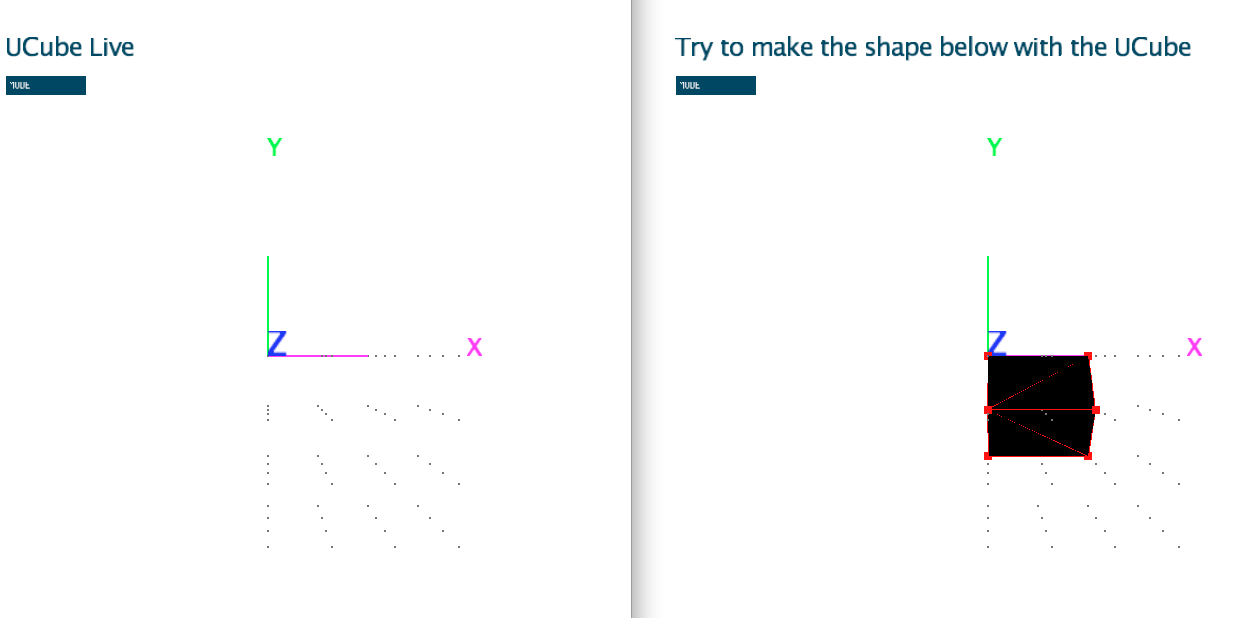
\includegraphics[width=.8\linewidth]{images/ucubescreentest}
\end{array}$
\end{center}
\caption{A screenshot of the testing setup, with the live output from the UCube
on the right and the target shape on the left.}
\label{fig:ucube_test1}
\end{figure}

Participants were instructed to place the poles on the board (but not shown
how), and were told that the software model could be rotated and filled in using
the keyboard and mouse, should that help them complete the task. The
participants were not given any hints as to how to complete the shapes and were
not told when they had the correct configuration (they had to indicate their
belief that the model was done). Participants were also instructed to 'think
aloud' about their actions. The main purpose of the pilot study was to get an
initial impression of how the UCube would act as an accessible 3D modeling
tool�how well it could help ``3D novices'' overcome the ``2D bottleneck''.

\subsection{Results and Discussion} 
Of the six groups who participated, four groups successfully modeled all five
shapes, one group ran out of time after three shapes, and one group finished one
shape. Sessions lasted between 17 and 30 minutes.
A variety of problem-solving strategies were observed during testing, as the
participants tended to treat the exercise as a sort of puzzle to be solved.
Simple methods equivalent to ``try and see'' were common, and seemed to serve as
a base point from which to draw conclusions about the relationship between the
3D model and 2D on-screen representation (e.g. ``No, not there, up one''). More
sophisticated strategies were also observed� ``deconstructing'' more complex
shapes into smaller, easier-to- model shapes (e.g. thinking of one side of a
cube as a square) was observed from several groups. Another popular technique
was to systematically match the on-screen perspective from the live model with
the shape they were attempting to model (e.g. ``Okay, first let's do the top
view, and then go from the side''). By orienting the two models similarly,
participants were able to make more accurate modeling decisions as well as check
their model against the on-screen shape. Counting distance in terms of spaces on
the board, between switches, or between dots on the screen was also a very
common technique of reasoning about and describing position. For example, by
counting that two vertices of a shape were separated by ``two dots over and one
down'' on the screen, subjects were able to count the distance out on the
physical UCube board. A few of the more mathematically-advanced participants
used terms such as ``axis'' and ``origin'' to orient themselves and describe
various positions on the board to their partners.
Another revealing observation in the pilot study was that, in the few instances
of mechanical failure (certain switches not lighting up, towers not plugging in
properly, or points not showing up on screen) the participants were still able
(with a high degree of certainty) to complete the assigned tasks. This appears
to indicate that, as opposed to arbitrarily moving the towers around until the
two sides of the computer screen looked the same, participants had formed a more
substantial mental model of the relationship between the UCube interface and the
2D representations on the screen. That opens the possibility that by performing
the embodied interactions necessary to operate the UCube, participants had
actually strengthened their understanding of how 3-dimensional space is
typically represented on a 2D screen. Although further testing and observation
is needed, this finding would strengthen the argument for using the UCube in an
educational setting to improve understanding of 3D space, as well as providing a
gateway for youngsters to move on to more complex modeling software.
While the variety of problem-solving techniques we witnessed is a testament to
the participants' ingenuity, it is also indicative of the fact that parts of the
UCube are not immediately intuitive. While none of the participants had trouble
understanding how to place the towers on the platform, the positions of the
towers and switches had to be reasoned out explicitly. It was common for groups
to clear the board of any poles when starting a new shape, even in cases where
an overlap of points or tower positions existed. (Figure XXXX, for example�shown
earlier in the context of explaining the UCube's operation�depicts one of the
students placing a tower and checking the screen to see whether the tower
placement is appropriate.) Although most groups completed all the shapes (or ran
out of time), there were some expressions along the way of the difficulty of the
task (e.g. ``This is hard'', or ``This is like a puzzle''). This indicates that
design changes can be made in future iterations to help clarify the
correspondence between positions on the UCube platform and the on-screen
representation; for example, labeling the both the physical and software grid
with a simple alphanumeric system.
Despite these drawbacks as well as the inherent limitations of the UCube design,
these early results indicate a promising ability of youngsters to effectively
engage with the UCube interface. In fact, despite various levels of success in
completing the assigned tasks, the vast majority of participants exhibited a
high level of engagement with the UCube. For example, although the group that
completed only one shape seemed unmotivated to attempt to model the other
shapes, they continued to play with the interface and observe the results, even
stating ``this is fun'' and ``I like the switches''. Participants also saw
potential uses for the UCube outside of the specific exercise we assigned.
Comments (unsolicited) included, ``you should use this to teach geometry'' and
``you could make this a puzzle game''.
At the very least, these early results indicate that the majority of
participants were able to take a 2-dimensional representation on the screen and
model its 3-dimensional equivalent using the UCube, a very encouraging result in
our eyes.

\section{Further UCube Study}

Early in 2012, we conducted a further user study of the UCube with a group of
11-13 year olds. The group consisted of ten participants, eight boys and two
girls, from a local middle school multimedia class. Every participant was
individually led through two separate exercises (outlined below) using the
UCube. 

\subsection{Procedure: Modeling}
Participants were handed a 3D-printed shape (modeled and printed from the UCube)
and were instructed to attempt to model the shape using the UCube. The
participant was initially allowed to hold the shape for approximately 10
seconds, after which they would hand the shape back to the facilitator and
attempt to model the shape from memory. Participants were instructed that they
may ask to hold the shape again, at which point they were allowed to hold it
throughout the duration of the modeling task. Additionally, users were
instructed that they had the option to skip a shape and return to it at a later
point in the exercise.
The five physical shapes presented were: a cube, a tetrahedron, a diamond, a
``house'' (a cube with a pyramid on top), and a complex irregular polyhedron.
The models were presented to the user starting with the cube (as this was deemed
to be the most basic shape with regard to modeling complexity). To avoid an
ordering bias, we randomized the presentation sequence of the next four shapes
using an online random order generator. If, after skipping a shape and returning
to it, the participant was still having difficulty, we offered them the
opportunity to attempt modeling the shape with the help of the UCube software,
the effects of which are discussed in the results section. Participants were
given a total of 25 minutes for the modeling exercise. We recorded, but did not
limit the modeling time per shape, only the total time for all five shapes.

\subsection{Procedure: Matching}
Participants were instructed to face away from the UCube while the facilitator
modeled a set of lights on the UCube corresponding to one shape among a set of
physical models laid out on the table next to the UCube.
Once the lights on the UCube were set up, the participant was instructed to turn
around, and indicate which physical object they thought the set of lights on the
UCube corresponded to.
There were nine physical models presented on the table, and consisted of a cube,
a tetrahedron, the �house� shape, a diamond, a triangular prism, an elongated
hexagon, a parallelogram, a trapezoid, and an irregular polyhedron (see
\ref{fig:ucube_shapes} for a picture of all the models). The shapes were
always presented on the table in the same order and orientation to avoid
discrepancies in perception or association.
Of the nine shapes, the participants were asked to match five of them (the cube,
the triangular prism, the parallelogram, the elongated hexagon, and the
trapezoid). Thus, only the cube was presented in both the matching and modeling
exercises. As with the modeling exercise, the cube was presented first, with the
remaining four shapes presented in a computer-generated randomized
order.Participants were given a total of ten minutes for the matching exercise,
corresponding to two minutes per shape, and were instructed to think aloud
during the process.

\begin{figure}[h]
\begin{center}$
\begin{array}{cc}
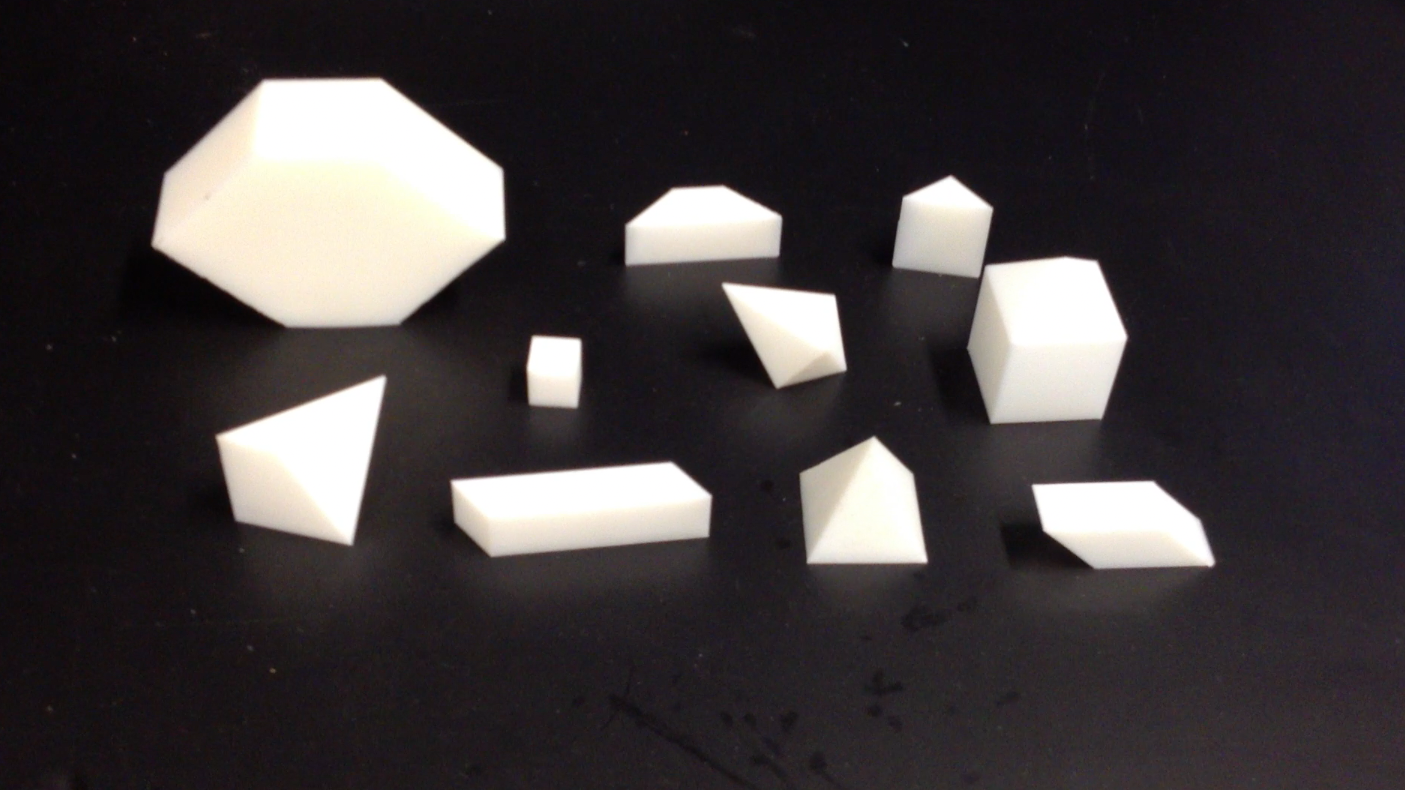
\includegraphics[width=.8\linewidth]{images/ucube_shapes}
\end{array}$
\end{center}
\caption{The nine models used during the user study:
diamond, trapezoid, parallelogram, cube, elongated hexagon, irregular 
polyhedron, triangular prism, tetrahedron, house.}
\label{fig:ucube_shapes}
\end{figure}


\subsection{Results} 
While many established forms of 3D modeling systems can be confounding and
operationally too complex for a child to navigate, the UCube was positively
received and system instruction was accomplished with just a minor introduction
and demonstration (system instruction and demonstration lasted approximately 2-3
minutes). We found this first instance of system comprehension to offer some
validation that the UCube worked well as a user-friendly 3D modeling device.
This section will detail the outcome of both the modeling and matching tasks
performed.

\subsubsection{Exercise 1: Modeling} 
Modeling occurred under three conditions:recreate the object from memory,
construction of the object while it was in the participant�s possession, and
modeling the shape with the help of the UCube software. Overall, 21 of 50 shapes
were completed from memory, 12 of 50 were completed while holding the shape, and a
further 8 of 50 were completed with the aid of the UCube software, for a total
of 41 out of 50 shapes modeled successfully (82\%). Of the nine missed shapes,
seven were of the same shape, the complex polyhedron. The remaining two misses
were from the same participant, who ran out of time before completion.
Of the 10 participants, 8 were able to recreate the cube from memory, whereas
only 4 were able to recreate the diamond and the tetrahedron from memory. Half
of the participants constructed the house from memory, and no participants were
able to complete the irregular polyhedron from memory. However, once shown the
software the majority of the participants found the modeling task significantly
easier to perform. The irregular polyhedron was by far the hardest shape and was
only able to be completed by 3 of the 10 participants either after continued
possession of the shape or using the software.

\begin{figure}[h]
\begin{center}$
\begin{array}{cc}
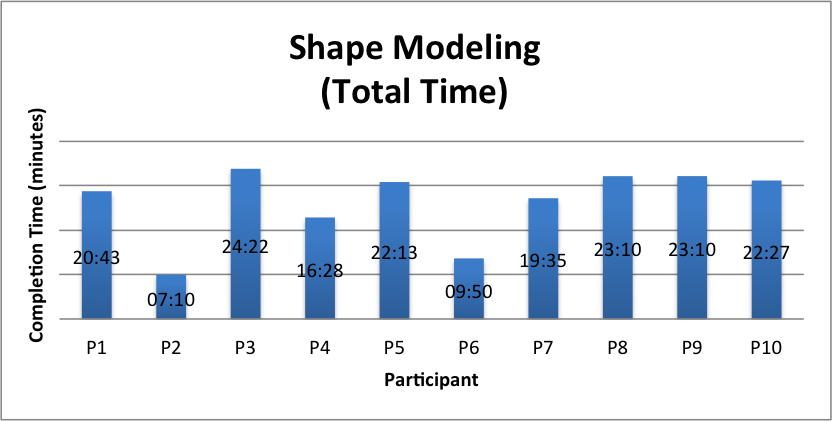
\includegraphics[width=.47\linewidth, height=1.75in]{images/modeling1}&
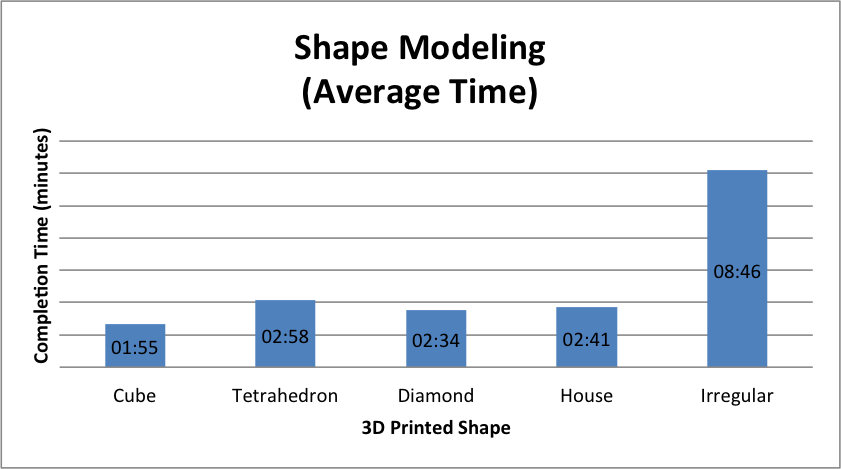
\includegraphics[width=.47\linewidth, height=1.75in]{images/modeling2}
\end{array}$
\end{center}
\caption{Results of the modeling task, showing total modeling time spent per
participant (left) and average modeling time spent per shape across
participants (right).}
\label{fig:modeling}
\end{figure}


\ref{fig:modeling} represents the total completion times per participant (on
the left) and average time per shape (right). Two exceptional completion times
were observed, where participants finished modeling all the shapes in under 10
minutes. However, the majority of participants finished the task in the 19-25
minute range. Only one of the participants ran out of time. Once participants
had been introduced to the software, 9 of 10 of participants were able to
complete all but the irregular polyhedron. It is interesting to note that of the
10 participants, the child that had the most difficult time modeling, the lowest
shape completion rate, and the longest completion time during the matching
exercise was the youngest participant.


\subsubsection{Exercise 2: Matching} 
Out of 50 matching tasks (five per participant), all but three tasks were
completed in 20 seconds or less. \ref{fig:matching} displays the total time
spent on the matching task per participant (left) and the average completion
times for each shape (right).
No participant selected the wrong shape (a few preliminary ``mis-selections''
were made that the participants quickly corrected), and all participants
completed the task in well under the allotted 10 minutes. The lack of errors in
the matching task is highly encouraging as a basis from which to reason about
youngsters' abilities to perceive and reason about convex hulls as a set of lit
vertices in space, meaning that this kind of 3D modeling interface might be
applied to other domains (e.g., as a cognitive assessment tool, a puzzle game,
etc.) with some optimism.

\begin{figure}[h]
\begin{center}$
\begin{array}{cc}
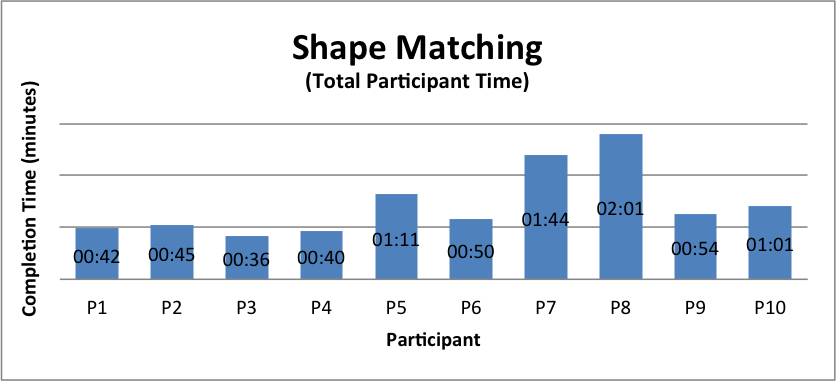
\includegraphics[width=.47\linewidth, height=1.75in]{images/matching1}&
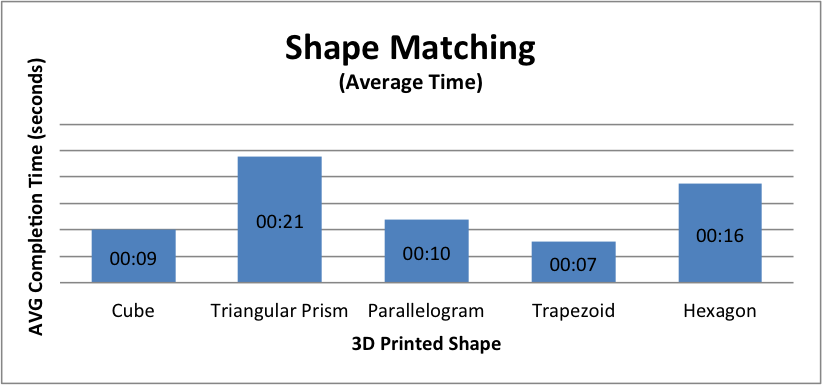
\includegraphics[width=.47\linewidth, height=1.75in]{images/matching2}
\end{array}$
\end{center}
\caption{Results of the matching task, showing total time spent per
participant (left) and average time spent per shape across
participants (right).}
\label{fig:matching}
\end{figure}


\subsubsection{Observations} 
Modeling trends as well as distinct modeling behaviors were documented in the
process. Common observations included building from the ground up (lowest
vertices first), building in the orientation that the object had been presented
in, not clearing the poles/lights from the UCube before starting to model a new
shape, and modeling a shape by breaking it up into discrete parts (e.g. a
participant building a house would commonly build a cube first and then add on a
vertex to the top; a participant constructing the diamond might combine two
opposite facing triangles.).

Unique behaviors were exhibited in the modeling process as well, reflecting a
type of user-specific construction-based problem- solving. One participant used
their arm to connect the red lights of the UCube for shape definition. A few
participants oriented the object differently than how it had been
presented�typically this occurred for the modeling of those objects with a
pyramidal apex (tetrahedron, house, diamond). Apex formation was perhaps one of
the most difficult concepts for most participants to grasp, as it required them
to strategically align the base on a 3x3 grid so there was a middle plug for
them to create the apex. If participants were fixated on designing from a 4x4
grid then there was no center plug for them to create a midpoint. Some
participants ended up building an oblong polyhedron as opposed to a cube, or an
oblique polyhedron as opposed to an equilateral tetrahedron. Other observed
behaviors included a participant who modeled shapes by turning on lights for an
entire shape edge, as opposed to just the corners and a participant who built
shapes that were floating, as opposed to resting on the base of the UCube.
There were also some notable behaviors regarding physical and gestural actions
of the participants. Many participants modeled with both hands simultaneously,
placing towers and flipping switches without a clear preference for a dominant
hand. Participants would often gesture with their arms following an arc in
parallel with a face of the object they were currently modeling. This ``tracing''
behavior was also noticed when participants were holding a physical model and
tracing a side of the object with their fingertip, often while rotating the
object with the other hand. Finally, during object possession phase three
participants actually placed the 3D object on top of the UCube in the modeling
space while they reasoned out the construction (see
\ref{fig:user_placedModel} for an example).

\begin{figure}[!ht]
\begin{center}
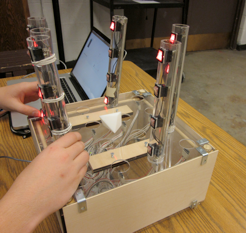
\includegraphics[width=.45\linewidth]{images/idc3}
\end{center}
\caption{A participant modeling with the UCube, using a strategy of placing the
physical model on top of the UCube while modeling, as well as using both hands
simultaneously to manipulate the towers.}
\label{fig:user_placedModel}
\end{figure}



\section{SnapCAD and PopCAD}

%- see
%http://silccenter.org/index.php/testsainstruments#MRT for the instruments, see
%http://www.spatialintelligence.org/publications_pdfs/Ehrlich\%20Levine\%20\%20Goldin-Meadow\%20\%282006\%29.pdf

Starting in early 2014 we conducted a study using both the SnapCAD and PopCAD
devices with a group of 11-18 year olds at a local drop-in enrichment program
focuses on children from under-served and low socioeconomic communities. Twenty
participants enrolled in the study, consisting of 12 boys and 8 girls (no one
responded with other, although it was an option). We collected some basic
demographic information, including age, race, grade level, 3D modeling
experience, 3D printing experience, computer ownership and use, interest in
engineering, and how difficult they thought classes in school were. 

To present these findings, then: the participants were primarily of
Latino/Hispanic descent, but also included those of African-American,
American-Indian, Asian, and Caucasian descent. Grade levels ranged from
6th-12th, with an overall average of 7.9 (8.33 for boys, 7.75 for the girls).
Average age was 14 years, 1 month, 20 days (14 years, 6 months for boys, 13
years, 7 months for girls). 16 of 20 participants had a computer at home.
Describing their comfort level using a computer on a scale from 1 to 10 (10
being most comfortable), the participants averaged 7.9 (8 for boys, 7.75 for
girls), with no scores below a 5. Of the participants who had a computer at
home, two reported using it only a few times a year, five used it a few times
per month, four used it a few times per week, and five reported using the
computer everyday. Only three of the participants had any experience with 3D
modeling software. Interestingly, only two of the participants had never heard
of 3D printing before enrolling in the study, but none of them had ever designed
or printed anything using a 3D printer. When asked about their interest in
engineering, only seven children (all boys) stated they were definitely
interested. However, only two kids (both girls) stated that they were definitely
not. The rest (11 kids) stated that they were either `maybe' interested, or `not
sure'. When asked how difficult they felt school classes were, six responded
`easy for me', 10 said `somewhat easy for me', and four responded `somewhat hard
for me' (no one responded `hard for me').


The study ran for seven weeks and comprised several stages, the first being a
pre-assessment of spatial reasoning skills. The spatial reasoning assessment was
done using the ``Children's Mental Transformation Task'' developed by Susan
Levine (\cite{ehrlich2006importance} p.1260-1261). In the task, participants are
shown two pieces of paper, side-by-side. One piece shows a geometric shape,
split apart and rotated in one of several different ways. All shapes were
symmetrical either horizontally or vertically, and thus split along either a
vertical or horizontal line of symmetry. Shapes were translated in one of four
different ways: (a) translated perpendicular to the line of symmetry (direct
translation), (b) translated and then moved diagonally apart (diagonal
translation), (c) rotated 45 degrees outward from the line of symmetry (direct
rotation), or (d) rotated and then moved diagonally apart (diagonal rotation).
The other piece of paper contained the geometric shape, recombined correctly,
along with three incorrect choices. In the study we conducted, participants were
given two sets of 10 shapes, one set as a pre-assessment before doing any
modeling, and another (completely different) set after completing the entire
study, as a post-assessment. Figure \ref{spatialTest} shows an example
instrument, with the four possible translations.

\begin{figure}[!ht]
\begin{center}
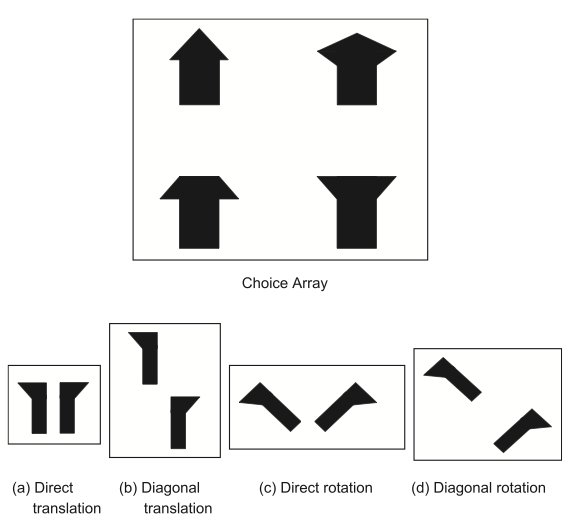
\includegraphics[width=.5\linewidth]{images/SpatialTestArray}
\end{center}
\caption{An example problem from the spatial reasoning exercise. The figure at
the top shows the choice array of four shapes, where the lower left figure is
the correct option. Examples (a) through (d) show the four different types of
translations found in the exercises - direct translation, diagonal translation,
direct rotation, and diagonal rotation.}
\label{spatialTest}
\end{figure}


After the pre-assessment, participants were split into two groups of ~10
students each - the selection alternated evenly based solely on order of
participation - with group A modeling first on the PopCAD and group B modeling
first on the SnapCAD (as described in Chapter 2). Each session proceeds roughly
as follows: a brief introduction to the device, during which the participant is
only told how to operate the device, but not what any of the buttons do, and
given free time to become comfortable with the interface. Participants were
encouraged to explore both the interface, and the buttons in the software that
control the three primary modeling modes (convex hull, path, minimal spanning
tree).

Once the subject indicates that they are ready to move on, we move into a series
of three modeling exercises that explore each of the aforementioned modes. The
basic operation and a brief explanation of each mode were given to the
participants as an introduction to each mode. Four 3D-printed models
representative of each mode were presented to the user in an order judged to be
from least complex to most complex (and thus was the same for each user), for a
total of 12 modeling tasks across the three modes. 24 models were used - one set
of 12 was used across every user's first session (independent of device), with a
remaining 12 models used in every user's second session. Figure XXXXX shows the
two sets of models side-by-side.

\begin{figure}[!ht]
\begin{center}$
\begin{array}{cc}
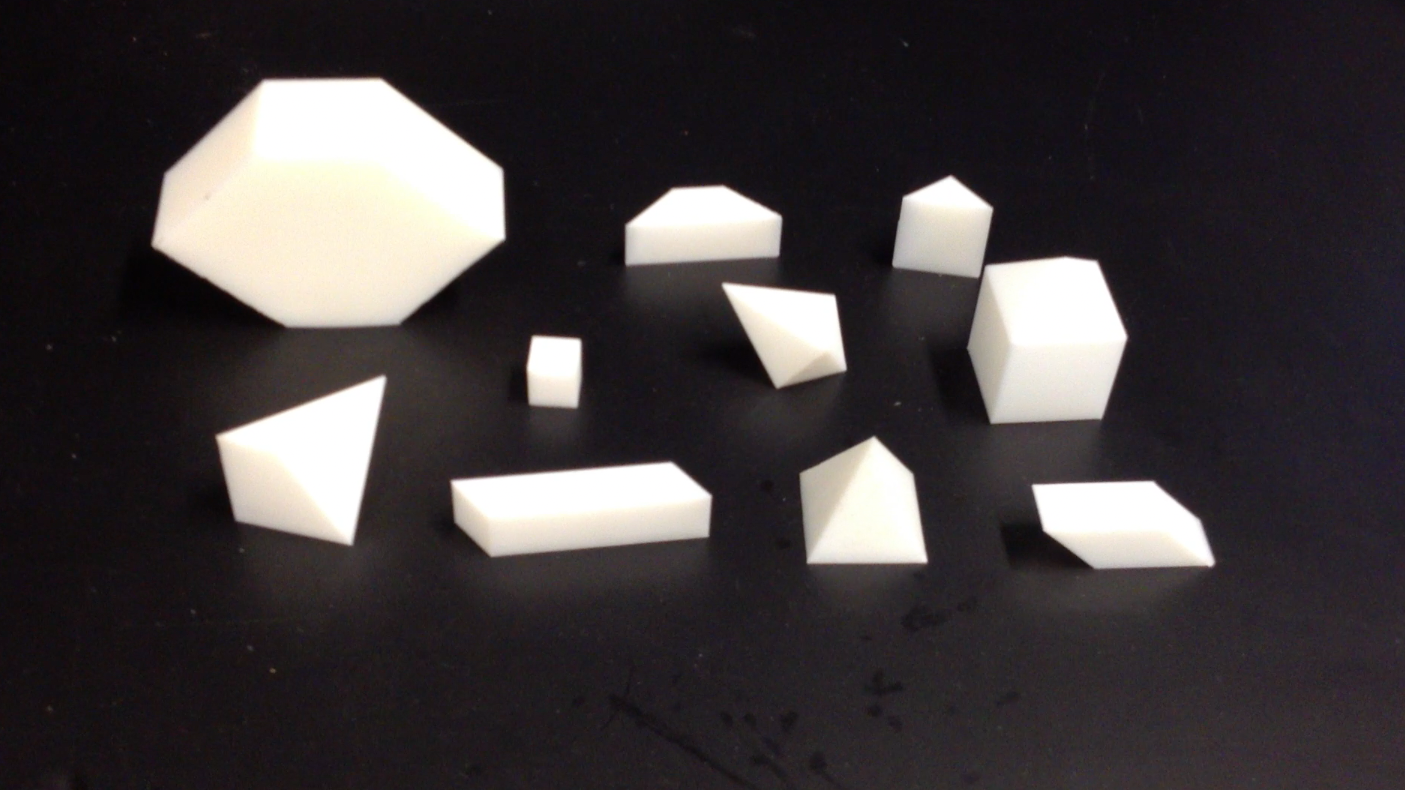
\includegraphics[width=.47\linewidth, height=1.75in]{images/ucube_shapes}&
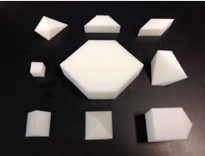
\includegraphics[width=.47\linewidth, height=1.75in]{images/studyshapes}
\end{array}$
\end{center}
\caption{The two groups of 12 3D printed models used in the first session
(left) and second session (right).}
\label{3dModel}
\end{figure}


The tasks that follow are the same for each device:

Task 1: Convex Hull Modeling

The participant will be given a brief demo of how the `convex hull' modeling
mode interprets the points from the device.  The user will then be presented
with a series of four (4) plastic, 3D-printed models that were modeled on the device
using �convex hull� mode. For each of these shapes, the participant will
attempt to recreate the shape using the modeling abilities of the device. The
user will be instructed to indicate when they believe they are done, as well as
to think aloud about their modeling process. Each modeling task will be capped
at ten minutes. The time to completion (of lack thereof), completion code,
observational notes, and video shall be recorded.

Task 2: Path Modeling

The participant will be given a brief demo of how the �path� modeling mode
interprets the points from the device. The user will then be presented with a
series of four (4) plastic, 3D-printed models that were modeled on the device
using the �path� mode. For each of these shapes, the participant will attempt to
recreate the shape using the modeling abilities of the device. The user will be
instructed to indicate when they believe they are done, as well as to think
aloud about their modeling process. Each modeling task will be capped at ten
minutes. The time to completion (of lack thereof), completion code,
observational notes, and video shall be recorded.

Task 3: Minimal Spanning Tree Modeling

The participant will be given a brief demo of how the �minimal spanning tree�
(aka �tree�) modeling mode interprets the points from the device. The user will
then be presented with a series of four (4) plastic, 3D-printed models that were
modeled on the device using the �tree mode. For each of these shapes, the
participant will attempt to recreate the shape using the modeling abilities of
the device. The user will be instructed to indicate when they believe they are
done, as well as to think aloud about their modeling process. Each modeling task
will be capped at ten minutes. The time to completion (of lack thereof),
completion code, observational notes, and video shall be recorded.

Task 4: Freehand Modeling

After the modeling tasks are complete, participants are invited to ``freestyle''
model an object of their choosing, using any of the three modeling modes. By
asking participants to think aloud about their intentions and thinking processes
during this exercise, we hope that a deeper understanding may be gained of the
strengths and weaknesses of the system, as well as the thought processes and
engagement of the users in attempting to model a specific model of their own
choosing. These saved models are analyzed, based on which mode was used to
create them, complexity (based on number of points used), and whether the shape
was `exploratory' or `intentional' (i.e., was the end artifact a result of sort
of happy accident, or the result of intentional process to create a specific
model).


For the first three modeling tasks (but not the freestyle modeling), time to
completion (or request to move on) is recorded, along with an outcome code. The
outcome is coded according to a set of conditions detailed below in table
\ref{modelingError}, and was developed upon analysis of the recorded video, in
an attempt to fit the sorts of repeated behaviors that were in fact observed.

\begin{table}[!ht]
\small
    \caption[Coding rubric used in analyzing modeling exercise outcomes.]{
	The coding used in analyzing the modeling exercise outcomes, based on
	observations from video taken during the study.}
    \begin{center}
    \begin{tabular}{| p{3.5cm} | p{1.0cm} | p{7.2cm} | } \hline
	$Category$ & $Code$ & $Definition$   \\ \hline
	Correct & C & A complete and correct modeling of the shape \\ \hline
	Error in recognition & E1 & The correct shape was modeled, but the user did not
	identify it \\ \hline 
	Error in belief & E2 & A belief that the modeled shape has been modeled
	correctly, when it has not \\ \hline 
	Error in implementation & E3 & User knew shape was incorrect, and gave a
	correct explanation \\ \hline 
	Error in strategy & E4 & Knew shape was incorrect, and did not know why or gave
	an incorrect explanation as to why \\ \hline 
	Error in proportion & EP & The general shape is correct, but the proportions in
	one or more dimensions is off (e.g. too tall, not wide enough, etc.) \\ \hline
	Incomplete & I & Participant ran out of time, gave up, or asked to move on \\
	\hline
	\end{tabular}
   \\ \rule{0mm}{5mm}
\end{center}
\label{modelingError}
\end{table}

Participants were asked to ``think aloud'' about their process, difficulties,
modeling choices, etc. In the case that the user believed they had correctly
modeled the shape (cases C and E2 in table \ref{modelingError}) they were asked
to explain their modeling strategy\footnote{Cases E1,E3,E4, and I did not
provide the grounds from which to ask about modeling strategy and so were not
recorded.}. Their explanation was videotaped and analyzed based on the coding
strategies laid out in ``The Importance of Gesture in Children's Spatial
Reasoning"(\cite{ehrlich2006importance}, p.1264), laid out in table
\ref{codingStrategy} below. The rationale for performing this analysis in based
in part on work by Ehrlich, Levine, and Goldin-Meadow
\cite{ehrlich2006importance}\cite{levine1999early}\cite{goldin2005hearing},
which suggests that the frequency of gesture and relationships between speech
and gesture act as a window into the learning state of the subjects.

\begin{table}[!ht]
\small
    \caption[Coding rubric for speech and gesture during user explanation of
    modeling strategy]{ The various coding strategies used in the video
    analysis of subjects' modeling strategy explanations. Borrowed and adapted
    from \cite{ehrlich2006importance}.}
    \begin{center}
    \begin{tabular}{| p{1.5cm} | p{4.2cm} | p{4.2cm} | p{4.2cm} |} \hline
	$Category$ & $Definition$ &   $Speech Examples$  & $Gesture Examples$ \\ \hline
	Movement & Any indication of movement & ``Just slide them together and then it
	looks like that'' & Miming movement with the hands\\ \hline 
	Perceptual Features & Focus on a particular feature of the model & ``Because
	there is a little bend in here and a point thing here'' & pointing to a
	specific feature on the model \\ \hline 
	Perceptual Whole & Any indication of seeing the model as a whole & ``It looks
	like an arrow!'' & Gesture indicating inclusion of the whole shape \\ \hline
	Vague & An expression of strategy that the coder cannot decipher & ``Because I
	looked at that and I looked at the differences'' & Waving gestures above the
	computer o device that do not indicate any specific strategy \\ \hline 
	Other & Any strategy not listed above & ``And here is like half of it.
	But so and two halves make a whole'' & Using the hand to form a straight line
	through the middle of the whole shape to represent the line of symmetry
	\\
	\hline
	\end{tabular}
   \\ \rule{0mm}{5mm}
\end{center}
\label{codingStrategy}
\end{table}


The second session is similar to the first, with the subject using the device
not used in session one, and with 12 new models. Once modeling on the second
device is completed, users will take a second spatial reasoning assessment of an
additional ten questions to help gauge if any meaningful difference in spatial
reasoning skills has occurred throughout the study. 

A slightly modified version of the software was used for the user study,
eliminating several of the functions not being evaluated for the sake of
presenting a clear interface for the users. The multiple hull modes, spline,
load, and save functions (described in Chapter 2) were eliminated, and the rest
of the graphical user interface was reorganized and streamlined. We
combined the three different .stl export buttons into a single export button
that handled all three modes, changed the order of the remaining buttons and
made them larger, and made the X,Y, and Z axis markings larger.

\subsection{Results}

This section reports on the results from our study, relaying our findings across
both sessions, genders, modeling modes, and spatial reasoning scores in an
attempt to tease out what conclusions, if any, we might make about the strengths
and weaknesses of our devices as well as how interacting with our devices
affected user's spatial reasoning abilities, 3D modeling skills, or congruence
between speech and gesture in explaining the cognitive learning state of the
user.

\subsubsection{Modeling Results}

In this section we will focus on delivering the results from the modeling
exercises - users went through two sessions, modeling 12 shapes each time (4
shapes each using convex hull, path, and minimal spanning tree modes) for a
total of 24 exercises. For each modeling task, a result code was recorded per
the rubric shown in table \ref{modelingError}. One user dropped out of the study
(user 6) before completing round one, leaving us to report on 19 users, 10 of
whom started on the PopCAD and 9 of whom started with the SnapCAD.

\begin{table}[!ht] 
\small
    \caption[Session One modeling results per participant]{ This table shows the
    total number of modeling tasks marked as correct (out of 12) broken down by
    participant, as well as the age, gender, and modeling device on which they
    worked.}
    \begin{center}
    \begin{tabular}{| c | c | c | c | c |} \hline
	$User$ & $Number Correct$ & $Age$ & $Gender$ & $Device$\\ \hline 
    1 & 11 & 14 & M & PopCAD \\ \hline
    2 & 6 & 12 & F & SnapCAD \\ \hline
    3 & 6 & 15 & M & PopCAD \\ \hline
    4 & 4 & 13 & M & SnapCAD \\ \hline
    5 & 5 & 12 & M & PopCAD \\ \hline
    7 & 12 & 15 & M & PopCAD \\ \hline
    8 & 4 & 12 & F & SnapCAD \\ \hline
    9 & 8 & 14 & M & PopCAD \\ \hline
    10 & 12 & 18 & F & PopCAD \\ \hline
    11 & 9 & 14 & M & SnapCAD \\ \hline
    12 & 4 & 17 & M & SnapCAD \\ \hline
    13 & 9 & 12 & M & PopCAD \\ \hline
    14 & 1 & 13 & M & SnapCAD \\ \hline
    15 & 1 & 13 & M & SnapCAD \\ \hline
    16 & 12 & 12 & M & PopCAD \\ \hline
    17 & 11 & 13 & F & PopCAD \\ \hline
    18 & 8 & 17 & F & SnapCAD \\ \hline
    19 & 4 & 11 & F & PopCAD \\ \hline
    20 & 0 & 13 & F & SnapCAD \\ \hline
	\end{tabular}
   \\ \rule{0mm}{5mm}
\end{center}
\label{codingStrategy}
\end{table}

Out of a possible 228 correct shapes, the group successfully modeled 127, or
roughly 56\%. Those users who started with SnapCAD performed 37 of 108 tasks, or
34\%, while those using the PopCAD device completed 90 of 120 tasks correctly,
for a success rate of 75\%. Girls completed 45 of 84 tasks (54\%), while boys
correctly completed 82 of 144 tasks (58\%). Individual scores ranged from 0 to
12 (perfect), with an overall overage of 6.68 correct shapes per user. Average
correct shapes per user was 4.11 for SnapCAD and 9.00 for PopCAD.


\begin{table}[!ht] 
\small
    \caption[Session one modeling results per shape]{ This table shows the
    number of correct models generated from a given shape, broken down by
    device, gender, and average modeling time spent on the shape. Session one
    results only.}
    \begin{center}
    \begin{tabular}{| c | c | c | c | c | c | c |} \hline
	$Shape$ & $Total$ & $PopCAD$ & $SnapCAD$ & $Average$ & $PopCAD$
	& $SnapCAD$ \\
	 & $Number Correct$ & $Only$ & $Only$ & $Modeling Time$ & $Only$ & $Only$
	 \\\hline 
	 Convex Hull 1 & 8 & 7 & 1 & 6:33 & 5:25 & 7:49 \\ \hline 
	 Convex Hull 2 & 13 & 9 & 4 & 4:34 & 3:03 & 6:15 \\ \hline 
	 Convex Hull 3 & 8 & 7 & 1 & 5:29 & 4:33 & 6:32 \\ \hline 
	 Convex Hull 4 & 11 & 7 & 4 & 4:52 & 4:31 & 5:14 \\ \hline 
	 Path 1 & 17 & 10 & 7 & 2:08 & 1:22 & 3:00 \\ \hline 
	 Path 2 & 14 & 9 & 5 & 4:39 & 3:24 & 6:02 \\ \hline 
	 Path 3 & 8 & 6 & 2 & 6:21 & 4:52 & 8:00 \\ \hline 
	 Path 4 & 9 & 7 & 2 & 4:12 & 1:56 & 6:43 \\ \hline 
	 Tree 1 & 12 & 8 & 4 & 2:10 & 1:10 & 3:17 \\ \hline 
	 Tree 2 & 8 & 6 & 2 & 2:25 & 1:08 & 3:51 \\ \hline 
	 Tree 3 & 8 & 5 & 3 & 3:11 & 1:29 & 5:04 \\ \hline 
	 Tree 4 & 11 & 8 & 3 & 4:24 & 3:12 & 5:43 \\ \hline
	 \em{Total} & 127 & 90 & 37 & 4:15 & 3:00 & 5:38 \\ \hline
	\end{tabular}
   \\ \rule{0mm}{5mm}
\end{center}
\label{codingStrategy}
\end{table}



\begin{table}[!ht] 
\small
    \caption[Modeling Times per user (overall)]{Modeling times per user over
    all modeling exercises in session 1.}
    \begin{center}
    \begin{tabular}{| c | c | c | c | c | c | c | } \hline 
    $Mode$ & $Combined$ & $Number$ & $PopCAD$ & $SnapCAD$ & $Girls$ &
    $Boys$ \\
    &  $Average Time$  & $Correct$ & $Only$     & $Only$ & & \\ \hline     
     Convex Hull &  21:30:21 & 40 / 76 &  30 & 10 & & \\ \hline 
     Path &  17:21:57 & 48 / 76 &  33 & 15 & & \\ \hline 
     Minimal Spanning Tree &  12:11:52 & 39 / 76 &  27 & 12 & & \\ \hline 
     Overall &  51:04:10 & 127 / 228 &  90 & 37 & 45 & 82 \\ \hline 
 
	\end{tabular}
   \\ \rule{0mm}{5mm}
\end{center}
\label{codingStrategy}
\end{table}



\subsubsection{Mental Transformation Task Results}


\subsubsection{Speech and Gesture Coding}






\subsection{Discussion}






